Based on the design principles, problems, and potential solutions outlined throughout \cref{sec:opal-motivation}, we present our design for an in-NIC, task-independent, online reinforcement learning system---\emph{\approachshort{} (\approach)}.
At a high level, \approachshort{} is designed to use the auxiliary compute exposed by general SmartNIC devices to offer low-latency online learning, scaling according to available on-chip resources at build time.
As the allocation of cores/chip area is set ahead of time by a framework or system administrator, \approachshort{}(-\Coopfw) agents enumerate themselves at runtime, during initialisation.

\begin{figure}
	\centering
	\begin{subfigure}{\linewidth}
		\centering
		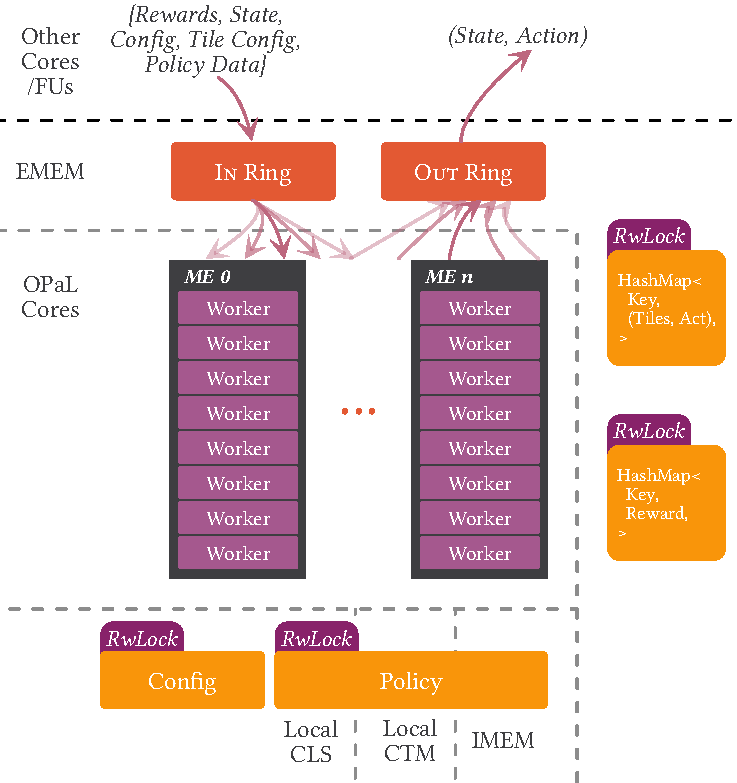
\includegraphics[keepaspectratio, width=0.78\linewidth]{diagrams/opal/ind}
		\caption{\Indfw{} (offline throughput-optimal). \emph{Workers} independently pull commands from (and push actions to) the environment, locking policy access for updates.\label{fig:single-and-parallel:single}}
	\end{subfigure}

	\begin{subfigure}{\linewidth}
		\centering
		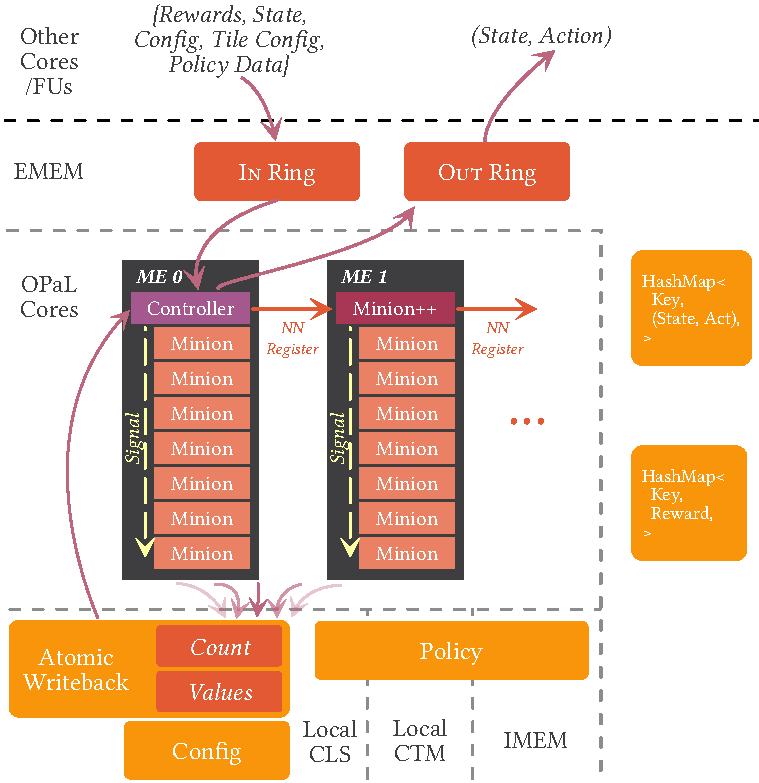
\includegraphics[keepaspectratio, width=0.8\linewidth]{diagrams/opal/coop}
		\caption{\Coopfw{} (online-optimal). A single \emph{controller} delegates RL computation and updates to many \emph{minion} threads, who operate on independent subtasks.\label{fig:single-and-parallel:parallel}}
	\end{subfigure}
	\caption{\approachshort{}'s compute strategies scale to fit device capacity according to either latency or throughput needs.\label{fig:single-and-parallel}}
\end{figure}

\Cref{fig:netro-arch,fig:single-and-parallel} outline our design and implementation on Netronome SmartNIC hardware in pursuit of this goal: unused device resources beyond the P4-PSA spec \emph{can and should be used} to drive asynchronous environmental control.
We explain relevant NFP architectural details later in \cref{sec:netronome-platform-fundamentals}.
\approachshort{} communicates with the packet pipeline of a P4 dataplane via \texttt{extern} plugins using \inring{} (state, configuration) and \outring{} (action) messages (\cref{fig:netro-arch}).
Internally, \approachshort{} either has all its cores act independently (\cref{fig:single-and-parallel:single}) or cooperate to solve each task (\cref{fig:single-and-parallel:parallel})---with different latency-throughput benefits (\cref{sec:action-and-update-computation}).
We open-source our firmware and control programs for the benefit of the community.\sidenote{\url{https://github.com/FelixMcFelix/pdp-rl-paper}}
Moving beyond the Netronome platform, we describe how our architecture may be adapted and improved on by bespoke hardware or FPGA-based deployment.

\subsection{System Model}
\approachshort{} is a general, task-independent framework for in-network, online training and execution of \emph{any reinforcement learning agent design} using classical methods.
\approachshort{} is agnostic to the meaning of state vectors it receives as inputs and the actions it produces, which are employed by other functional units or the dataplane.
However, in-NIC/in-network execution specifically benefits packet-, flow-, and network-level learning, control, and optimisation tasks.

\approachshort{} runs on one or more cores of a SmartNIC to convert fixed-point state measurements from the environment into a stream of actions using a stored policy.
As an example, this might be to map flow state and performance measurements into a queueing priority for future packets from that flow, or to compute and apply a rate limit to preserve quality of service.
These dedicated cores are then responsible for processing requests, computing actions, and updating the underlying policy in real time.
Combined with reward measurements, this policy can then be updated or trained from scratch entirely on the NIC, acting as a fully online RL agent.
An input state vector \emph{always} induces an action and, if desired, updates the policy using either an included reward or one retrieved from memory according to a (configurable) key placed alongside the state.
This allows for simultaneous control and learning over independent systems by the same agent (i.e., optimising several flows with their own reward measures, such as DDoS mitigation in an AS where each next-hop AS might have their own `health' metric).

%However, high-speed data networks impose inviolable per-packet deadlines.

To protect traffic throughput and allow effective deployment in as many environments as possible, \approachshort{} places RL execution on-chip, \emph{but off the main packet path}, communicating and running parallel to the main P4 dataplane.
As shown in \cref{fig:netro-arch}, this asynchrony allows coexistence with P4 programs, and imposes minimal impact on carried traffic for both bump-in-the-wire deployments and at end-points.
For instance, in the default deployment of a P4 packet processing pipeline on Netronome NFP chips several cores go unused (as does spare area on an FPGA design), making this paradigm possible.

%The main interaction model is that platform-specific IPC (message rings) is used to \emph{push} configuration, state vectors, and reward measurements to the RL system.
%These same mechanisms are used by other cores on the same device to \emph{pull} output actions from the RL system.
%Both input and output can occur on any other core of the device, i.e., as part of P4 \texttt{extern} plugins or a dedicated flow state measurement subsystem, while the P4 control plane itself provides granular control over which flows are monitored or affected.
%
%Runtime reconfiguration and interaction occur via the control and/or dataplane: the ease of use of the P4 pipeline's match-action tables and custom protocol parsers, combined with the dedicated input pipe to the NIC's controller (the host machine), allow these to be cleanly separated or combined as needed.
%Bit depth of quantised measurements/preferences, maximum policy sizes, and parallelisation strategy may be configured at compile time.

\subsection{Action and Update Computation}\label{sec:action-and-update-computation}
\approachshort{} applies the insights of \textcite{DBLP:journals/firai/TravnikMSP18} to minimise action latency; an action is computed, sent out into the environment, and only then is the underlying policy updated.
Using one of the below strategies chosen at compile time, a state vector is tile coded, converted into action probabilities, and an action is chosen.
This is then written out to the environment as in \cref{sec:agent-environment-communication}.
If online learning is enabled, \approachshort{} then checks an internal hashmap for a previous state-action pair matching the current instruction source, and if found then the policy is updated.
Updates are computed using \emph{single-step semi-gradient Sarsa}~\cite[pp. \numrange{217}{221}]{RL2E}, though modification to support other single-step methods would be trivial.
The new state- or tiles-action pair is then written into storage.
\approachshort{} can be configured to automatically select values of the input state vector as keys for state and reward storage.

Two firmware models govern how the compute-heavy parts of these tasks (action selection, policy updates) are carried out:
\begin{description}
	\item[\Indfw{} (\cref{fig:single-and-parallel:single})] Separate threads listen for new states, and each performs its work sequentially. Computing an action list requires a \emph{read lock} on the policy. If an update occurs, the core requests a \emph{write lock} before updating, greatly limiting online throughput. \emph{Tile lists} are stored for update computation.
	\item[\Coopfw{} (\cref{fig:single-and-parallel:parallel,alg:parsa})] Threads cooperate on processing state vectors, minimising latency. \emph{Minion} threads have a fixed list of work items, while a \emph{controller} thread sends compute/update commands before awaiting worker completion. Work items are disjoint, requiring no policy locks. \emph{State vectors} are stored for update computation.
\end{description}
Each offers a different point of optimisation; if updates are disabled, then the \indfw{} model can maximise throughput, while the \coopfw{} model is designed to minimise decision latency and needs no locks to update the policy (increasing \emph{online learning} throughput).
These correspond to only executing a trained policy and actively (re-)training a policy, respectively.
%ParSa is described here at a high level, as an algorithm suited for \emph{any multiprocessor environment}.
%We omit the simple logic for $\epsilon$-greedy action selection (which we implement), and note that modification to other single-step algorithms such as \emph{Q-learning} would be trivial.
%We detail our communication primitives in \cref{sec:intra-agent-communication}, and our work scheduling strategy in \cref{sec:work-allocation}, eliding the details of tile-coding as they are well-understood.
%In general it is also possible for the \emph{Ctl} task to act as an additional \emph{Minion} in its parallel sections; we were limited here by code store requirements on the NFP.
Latency and throughput, as in many networked systems, have different effects upon RL agents according to their design and target problem.
Higher RL throughput is a necessity for per-flow or per-packet applications, which can require high decision-per-second rates even after combining state measurements received from the environment, such as flow control in DDoS prevention.
Equally, lower latency affords an agent finer-grained control and learning of a problem, being able to react sooner to new information (e.g., device state in a routing optimisation problem, or queue depth when trying to enforce packet pacing).

Paradoxically, we found that in the general \emph{ParSa} algorithm it was more efficient \emph{to do more work} by having each worker recompute its tile subset from a stored state.
It transpired that cacheing this data placed a larger \texttt{memcpy} in the serial section, whose size did not scale at all with bit depth.
Additionally, we do not use bitshifts in place of division operations in our implementation, due to the strict limits that power-of-two tile widths place upon policy design.

\subsection{Agent-Environment Communication}\label{sec:agent-environment-communication}
\approachshort{} uses \emph{multiple-producer/multiple-consumer} (MPMC) messaging channels to communicate with other elements; be they P4 programs on the packet path, or other on-chip analysis and control modules.
Through these channels a system \emph{pushes} state vectors, reward measures, and setup packets as inputs, and \emph{pulls} a stream of state-action pairs as outputs.
This allows decisions to be made asynchronously---preventing packet stalling---and allowing many RL agents to be used if desired.
The key insight of this mechanism is that on-chip reward/state signals enjoy first-class support in the same manner as packets from the P4 dataplane, allowing agents to act on environmental signals from other on-NIC/chip asynchronous processes or the controller.
As such, \approachshort{} can receive input from P4 \texttt{extern}s or other, dedicated off-path flow state measurement applications.

Our implementation uses platform-specific IPC (\emph{EMEM ring buffers}) with hardware signalling on work arrival to achieve this.
As PDP hardware lacks dynamic memory allocation, P4 pipeline threads request buffers for packet payloads using a shared freelist to enable state/configuration/policy data handover.
Packet headers are extracted and parsed using the tooling autogenerated by the P4 pipeline.
We found that this costs a median \qtyrange{126}{140}{\nano\second} communication time (local--remote), comparable to message channels in the Rust and Go languages on commodity hardware.

%The main interaction model is that platform-specific IPC (message rings) is used to \emph{push} configuration, state vectors, and reward measurements to the RL system.
%These same mechanisms are used by other cores on the same device to \emph{pull} output actions from the RL system.
%Both input and output can occur on any other core of the device, i.e., as part of P4 \texttt{extern} plugins or a dedicated flow state measurement subsystem, while the P4 control plane itself provides granular control over which flows are monitored or affected.

\subsection{Intra-Agent Communication}\label{sec:intra-agent-communication}
Even with parallel problems such as \emph{ParSa}, optimising for latency requires meticulous care in how work is passed out and aggregated.
This is truer still when moving from the moderately fine-grained control of classical RL ($\sim$\qty{1}{\milli\second}) to its logical limit (tens of \si{\micro\second}).
Ordinarily, the marshalling of requests, responses, and shared data access can incur significant overheads.
On-chip execution and the nature of action preference computation allow us to use lockless atomic aggregation, removing the overheads of explicit messaging/packetisation.
Moreover, adjacent functional units/cores often have special-purpose shared registers or share a small fast cache to accelerate communication.

%?? reduce below and make take-homes more generic if possible

Our implementation exploits the locality of cores in the NFP, which can be factored into designs on other platforms like NetFPGA.
Policy compute/update/configure tasks are passed between cores using direct \emph{next neighbour} registers, signalling all child threads in response.
Such on-chip signals cost just $\sim$\qty{20}{\nano\second} per relayed message.
Each core performs atomic adds to a shared preference list and an acknowledgement counter checked by the master thread, implementing our wait-free \emph{ParSa} algorithm (\cref{alg:parsa}).
This is essential for aggregation compared to the use of bounded message buffers, which caused significant head-of-line blocking.

%On-chip local messages cost us just $\sim$\qty{20}{\nano\second} latency per relayed message
%
%In earlier designs we had experimented with bounded buffers as in \cref{sec:agent-environment-communication} for this, modified to be located solely in CLS memory, dedicating the master thread to result aggregation.
%We found that this created a performance bottleneck at this final stage, causing significant head-of-line blocking for each of the workers.
%Similarly, our next neighbour work notification scheme ($\sim$\qty{20}{\nano\second} latency per relayed message) was examined against \emph{reflector} and \emph{work queue} IPC mechanisms (\qtylist{58;126}{\nano\second} per messaged core).
%These slower messages can be used in theory to skip ahead into longer ME chains.

%Our implementation exploits the locality of threads, cores, and their parent islands in the NFP architecture.
%Policy compute/update tasks and configuration updates are passed between cores using these direct \emph{next neighbour} registers, signalling all child threads in response.
%Each task performs atomic adds to a shared preference list, and atomically increments an acknowledgement counter to be periodically checked by the master thread, implementing the wait-free \emph{ParSa} algorithm we introduce (\cref{alg:parsa}).

%In earlier designs we had experimented with bounded buffers as in \cref{sec:agent-environment-communication} for this, modified to be located solely in CLS memory, dedicating the master thread to result aggregation.
%We found that this created a performance bottleneck at this final stage, causing significant head-of-line blocking for each of the workers.
%Similarly, our next neighbour work notification scheme ($\sim$\qty{20}{\nano\second} latency per relayed message) was examined against \emph{reflector} and \emph{work queue} IPC mechanisms (\qtylist{58;126}{\nano\second} per messaged core).
%These slower messages can be used in theory to skip ahead into longer ME chains.

\begin{algorithm}
	\caption{ParSa---\emph{Par}allel \emph{Sa}rsa\label{alg:parsa}}
	\SetKw{Let}{let}
	\SetKw{Enum}{enum}
	\SetKw{In}{in}
	\SetKw{Await}{await}
	\SetKw{Const}{const}
	\SetKwProg{parsa}{Function \emph{ParSa}}{}{end}
	\SetKwProg{control}{Function \emph{Ctl}}{}{end}
	\SetKwProg{minion}{Function \emph{Minion}}{}{end}
	\SetKwProg{tilecode}{Function \emph{TileCode}}{}{end}
	
	\tcc{Given message passing mechanisms \emph{scatter} and \emph{recv}, quantised arithmetic functions $Q_\mathit{mul}$ and TileCode, and omitting schedule/config/precache updates.}
	\tcc{\emph{cfg}.$\alpha$, \emph{cfg}.$\gamma$ are hyperparameters affecting the significance of each update and the degree of forward-planning, respectively.}
	
	\Enum Par \{ Act(\emph{state}), Upd(\emph{delta, action, state}) \}\;
	\Const \emph{cfg, policy} = /* ... */\;
	
	\Let \emph{values}: [AtomicI32; \emph{cfg.n\_actions}] = \{0\}\;
	\Let \emph{acks}: AtomicI32 = 0\;
	\parsa{id, schedule}{
		\uIf{id==0}{
			\ForAll{state\_pkt \In \inring{}}{
				Ctl(\emph{state\_pkt})\;
			}
		}
		\Else{
			\While{true}{Minion(\emph{schedule}[$\mathit{id}- 1$], recv())\;}
		}
	}

	\control{state}{
		\emph{values, acks} = \{0\}, scatter(Par::Act(\emph{state}))\;
		acquire slot for \outring, copy \emph{state} into slot\;
		\Await acks == \emph{cfg.n\_minions}\;
		\Let \emph{action} = argmax(\emph{values})\;
		write \emph{action} into \outring{} slot, enqueue\;
		\If{cfg.online}{
			\Let \emph{((l\_state, l\_act, l\_val), found\_s)} = \emph{cfg}.lookup\_state\_from\_key(\emph{state})\;
			\Let \emph{(reward, found\_r)} = \emph{cfg}.lookup\_reward\_from\_key(\emph{state})\;
			\If{found\_s \&\& found\_r}{
				\Let $\delta_t$ = $\mathit{reward} + Q_\mathit{mul}$(\emph{cfg}.$\gamma$, \emph{values}[\emph{action}]) $-$ \emph{l\_val}\;
				$\delta_t$ = $Q_\mathit{mul}$(\emph{cfg}.$\alpha$, $\delta_t$)\;
				\emph{acks} = 0, scatter(Par::Upd($\delta_t$, \emph{l\_act}, \emph{l\_state}))\;
				\Await acks == \emph{cfg.n\_minions}\;
			}
			\emph{cfg}.store\_state(\emph{state}, \emph{action}, \emph{values}[\emph{action}])\;
		}
	}

	\minion{tasks, msg}{
		\Switch{msg}{
		\uCase{Par::Act(\emph{s})}{
			\ForAll{task \In tasks}{
				\Let \emph{hit} = TileCode(\emph{s}, \emph{task})\;
				\For{i \In [0..cfg.n\_actions)}{
					\emph{values}[\emph{i}].atomic\_add(\emph{policy}[\emph{hit}][\emph{i}])\;
				}
			}
		}
		\uCase{Par::Upd($\delta$, \emph{a}, \emph{s})}{
			\ForAll{task \In tasks}{
				\Let \emph{hit} = TileCode(\emph{s}, \emph{task})\;
				\emph{policy}[\emph{hit}][\emph{a}] += $\delta$\;
			}
		}
		}
		\emph{acks}.atomic\_add(1)\;
	}

%	\tilecode{state, task}{
%		\Let \emph{hit} = \emph{cfg}.get\_task(task)\;
%	}
\end{algorithm}

\subsection{Reconfigurability}
\approachshort{} allows policy design and algorithmic learning parameters to be changed at runtime using at most two control packets.
For instance, design changes are useful at the end of learning (moving from online to offline), or when trying to train a new policy for another problem from the same vantage point.
Parameter changes are useful when an online agent must become more (or less) adaptive to new data (i.e., after detecting a changepoint in traffic).
This extends to policy data, which may be imported from a pre-trained model via such packets and exported via PCIe to the host machine.
Some aspects must be chosen at compile time; bit depth, \Coopfw/\Indfw, and maximum policy/tiling/state sizes---these govern core operation or allocated memory.
Choosing a bit depth of \qtylist[list-pair-separator = { or }]{16;8}{\bit} halves/quarters policy memory costs, allowing more complex problems to be modelled using more dimensions or fine-grained tiles.

In our implementation, configuration packets are carried over UDP and signalled to the P4 parser using a reserved (pool 2~\parencite{rfc2474}) DSCP value as used by \textcite{DBLP:conf/isca/LiLYCSH19}.
While this mainly automates parser generation, it also allows for configuration to be received from only trusted hosts (over the dataplane if needed) via P4 rules.
Our control packet generation library and evaluation frameworks which build upon it are written in Rust.

%Runtime reconfiguration and interaction occur via the control and/or dataplane: the ease of use of the P4 pipeline's match-action tables and custom protocol parsers, combined with the dedicated input pipe to the NIC's controller (the host machine), allow these to be cleanly separated or combined as needed.
%Bit depth of quantised measurements/preferences, maximum policy sizes, and parallelisation strategy may be configured at compile time.

\subsection{Work Allocation}\label{sec:work-allocation}
Due to the lack of dynamic memory allocation on PDP hardware, and to simplify value lookups, policies cannot be stored sparsely.
As a consequence, tiling space requirements scale exponentially with dimension count, and so higher-dimension tilings must be placed in larger (and slower) memory regions.
As a result, in many architectures policy parameters are split across such regions, giving different access and compute costs to different tasks.

We use a simple first-fit work placement algorithm run in \approachshort{}, placing the largest work item into the least loaded thread of the least loaded core (as the NFP uses hardware threads).
Each work item is a separate \emph{tiling} over a list of dimensions, noting that many such tilings may be grouped into a set (using different offsets for smoother coverage of the state space).
The cost of any work item (from its dimension count and memory location) was empirically measured offline, and we weigh the total cost per core based on the number of minion threads available.
This weighting specifically accounts for the controller thread on the first core.
Work allocation and cached per-item data are recomputed when policy configuration is installed or changed.
Naturally, for $n$ tilings and $m$ threads this procedure is $\mathcal{O}{\left(n\log{m}\right)}$: two find/update min operations into binary heaps per tiling, storing $m/8$ and $\le8$ costs respectively.

%\subsection{Variable Quantisation Bit Depth}
%At compile-time, \approachshort{} can be configured to use \qtylist[list-final-separator = { or }]{32;16;8}{\bit} values in input states and its internal policies.
%Naturally, smaller bit depths reduce the storage required for policies, tiling data, and stored state-action pairs---allowing more complex problems to be modelled using more dimensions or fine-grained policies.
%Through the lens of computational efficiency, reduced bit depth should allows action preference lists to be read using fewer I/O operations (as more values may fit into a single machine word).
%
%We had investigated bit-stuffing several such values into a single word for our atomic writeback mechanism (as the platform offers both \qtylist{32;64
%}{\bit} atomic addition).
%This is analogous to SIMD---through clever use of padding bits---but we found that manipulating tiles into the correct format added \qty{10}{\percent} extra overhead.
%We investigate further performance implications of changing bit depth in the sequel.

%Potential: low-latency train for some specific points, and high throughput for others? Think on the exact note I took...
%
%``can have accel'd offline, train online subset w/ my approach''
%
%THis might mean "do 32-bit online", then downsample to 8-bit policy for high-throughput mode.
%
%Can changes in trained policy be used to transfer to a more complex function approximator elsewhere?

\subsection{Limitations}\label{sec:limitations}
Unfortunately, direct rule installation into P4 tables from the SmartNIC itself is not, in general, possible.
To achieve line-rate match-action table lookup, platforms like NFP use accelerated datastructures (e.g., DCFL~\parencite{DBLP:conf/infocom/TaylorT05}) which must be computed by the controller over the \emph{entire rule set}.
Even through \texttt{extern}s, directly adding new rules is neither feasible nor safe.
We instead suggest on NFP chips that \texttt{extern}s or datapath stages which apply RL actions to packets should maintain a small store of state-action pairs, and periodically send these back to the controller for batch installation.
This ensures that the majority of installed rules exhibit accelerated performance, while preventing installation delay on the newest decisions.
Platforms such as Intel Tofino greatly simplify this, with Tofino Native Architecture intrinsics such as \emph{Action Profiles/Selects} allowing a P4 action to be chosen based on a register value (i.e., an RL action).

%As is expected of parallel algorithms, efficient division of work, communication, and aggregation add per-task overheads in both the serial and parallel portions.
Efficient division of work, communication, and aggregation add per-task overheads in both the serial and parallel portions.
Even in wait-free algorithms, this requires a minimum number of workers to improve upon the latency bounds of a serial approach.
We investigate the exact worker count requirements imposed to break even or improve upon single-threaded execution in \cref{sec:results}.

\subsection{Targeting other device classes}
While this design caters to Netronome devices, many aspects have clear analogues in other SmartNICs, such as the NetFPGA SUME.
For instance, additional off-path functional units can serve as workers, like the floating-point adders used by \textcite{DBLP:conf/isca/LiLYCSH19}.
Rather than general-purpose IPC, \approachshort{} would be hard-wired between internal workers and to the P4$\rightarrow$NetFPGA~\parencite{DBLP:conf/fpga/IbanezBMZ19} actions that interface with it.
%Further optimisations arise from this model: a NetFPGA design would be able to replicate and optimise further on this concept of dedicated, low-latency communication between functional units.
As we show later, using a bit depth below the native word size reduces overall efficiency.
%This reduces overall efficiency even though considerably fewer reads are made.
We expect an FPGA design would allow this to match the desired bit depth and enable the SIMD-like optimisations we discuss without creative and costly bit-stuffing.

Bringing \approachshort{} to PDP switches such as the Tofino is difficult as they closely match the P4-PSA, leaving no spare general-purpose compute units.
Taking inspiration from real-time programming, a potential solution is to divide RL processing across several packets (i.e., computing a portion of the preference list each time) until further work would delay outbound transmission.
This would introduce new issues in concurrent access, work splitting, and altered timescales for learning: we leave their treatment to future work.

%While specifics of this design cater to Netronome devices, many aspects have clear analogues in NICs of similar form-factor, such as the NetFPGA SUME platform.
%For instance, other cores can be introduced by designing additional off-path functional units,  like the floating-point adders used by \textcite{DBLP:conf/isca/LiLYCSH19}.
%Rather than general-purpose IPC, \approachshort{} would be hard-wired between internal workers and to the custom actions that interface with it, using the P4$\rightarrow$NetFPGA toolchain to offer granular control over packet and flow selection.
%%Further optimisations arise from this model: a NetFPGA design would be able to replicate and optimise further on this concept of dedicated, low-latency communication between functional units.
%As our later results show, using a bit depth below the native word size forces the compiler to emit excess code to extract and re-align preference values, reducing overall efficiency.
%%This reduces overall efficiency even though considerably fewer reads are made.
%We expect that a more bespoke hardware/FPGA design would allow this to match the desired bit depth and enable SIMD-like optimisations we discuss without creative and costly bit-stuffing.
%
%Bringing \approachshort{} to high-port density devices such as Tofino-powered switches is more difficult.
%As discussed in \cref{sec:motivation}, Tofino ASICs map closely to the P4 PSA, meaning that there are no spare asynchronous general-purpose compute units to place this work on.
%Taking inspiration from real-time programming techniques, a potential solution is to divide RL actions across several received packets (i.e., iteratively computing a portion of the action preference list each time) until any further work would delay outbound transmission.
%This, however, would introduce new issues surrounding concurrent accesses, work splitting, and altered timescales for learning: we leave their treatment and examination to future work.
